\documentclass[a4paper,12pt]{article} % добавить leqno в [] для нумерации слева
\usepackage[a4paper,top=1.3cm,bottom=2cm,left=1.5cm,right=1.5cm,marginparwidth=0.75cm]{geometry}
%%% Работа с русским языком
\usepackage{cmap}					% поиск в PDF
\usepackage{mathtext} 				% русские буквы в фомулах
\usepackage[T2A]{fontenc}			% кодировка
\usepackage[utf8]{inputenc}			% кодировка исходного текста
\usepackage[english,russian]{babel}	% локализация и переносы

\usepackage{graphicx}

\usepackage{wrapfig}
\usepackage{tabularx}

\usepackage{hyperref}
\usepackage[rgb]{xcolor}
\hypersetup{
colorlinks=true,urlcolor=blue
}
\usepackage{multirow}
\usepackage{hhline}


%%% Дополнительная работа с математикой
\usepackage{amsmath,amsfonts,amssymb,amsthm,mathtools} % AMS
\usepackage{icomma} % "Умная" запятая: $0,2$ --- число, $0, 2$ --- перечисление

%% Номера формул
\mathtoolsset{showonlyrefs=true} % Показывать номера только у тех формул, на которые есть \eqref{} в тексте.

%% Шрифты
\usepackage{euscript}	 % Шрифт Евклид
\usepackage{mathrsfs} % Красивый матшрифт

%% Свои команды
\DeclareMathOperator{\sgn}{\mathop{sgn}}

%% Перенос знаков в формулах (по Львовскому)
\newcommand*{\hm}[1]{#1\nobreak\discretionary{}
{\hbox{$\mathsurround=0pt #1$}}{}}

\begin{document}
	
	\begin{titlepage}
	\begin{center}
		{\large МОСКОВСКИЙ ФИЗИКО-ТЕХНИЧЕСКИЙ ИНСТИТУТ (НАЦИОНАЛЬНЫЙ ИССЛЕДОВАТЕЛЬСКИЙ УНИВЕРСИТЕТ)}
	\end{center}
	\begin{center}
		{\large Физтех-школа электроники, фотоники и молекулярной физики}
	\end{center}
	
	
	\vspace{4.5cm}
	{\huge
		\begin{center}
			{Лабораторная работа 2.2.6}\\
			Определение энергии активации по температурной зависимости вязкости жидкости
		\end{center}
	}
	\vspace{2cm}
	\begin{flushright}
		{\LARGE Салтыкова Дарья \\
			\vspace{0.5cm}
			Б04-105}
	\end{flushright}
	\vspace{8cm}
	\begin{center}
		Долгопрудный 2022
	\end{center}
\end{titlepage}

\section{Введение}

\textbf{Цель работы:} 1) измерение скорости падения шариков при разной температуре жидкости; 2) вычисление вязксоти жидкости по закону Стокса и расчет энергии активации. 

\medskip

\noindent \textbf{Оборудование:} стеклянный цилиндр с исследуемой жидкостью (глицерин); термостат; секундомер; горизонтальный компаратор; микроскоп; мелкие шарики (диаметром 1-2 мм).

\section{Теоретические сведения}

\subsection{Энергия активации}
	
\noindent Двойственный характер свойств жидкостей связан с особенностя- ми движения их молекул. В газах молекулы движутся хаотично, в их расположении отсутствует порядок. В кристаллических твердых телах частицы колеблются около определенных положений равновесия — узлов кристаллической решетки. В жидкостях, как и в кристал- лах, каждая молекула находится в потенциальной яме электрического поля, создаваемого окружающими молекулами. Молекулы колеблются со средней частотой, близкой к частоте колебаний атомов в кристаллических телах ($\sim 10^{12}$ Гц), и с амплитудой, определяемой размерами объема, предоставленного ей соседними молекулами. Глубина потенциальной ямы в жидкостях больше средней кинетической энергии колеблющейся молекулы, поэтому молекулы колеблются вокруг более или менее стабильных положений равновесия. Однако у жидкостей различие между этими двумя энергиями невелико, так что молекулы нередко выскакивают из <<своей>> потенциальной ямы и занимают место в другой.

\medskip
	
\noindent Для того чтобы перейти в новое состояние, молекула должна преодолеть участки с большой потенциальной энергией, превышающей среднюю тепловую энергию молекул. Для этого тепловая энергия молекул должна — вследствие флуктуации — увеличиться на некоторую величину $W$ , называемую энергией активации. Температурная зависимость вязкости жидкости при достаточно грубых предположениях можно опистаь формулой

	\begin{equation}
		\eta \sim A e^{W/kT}
	\end{equation}
	
\subsection{Формула Стокса}
	
\noindent На всякое тело, двигающееся в вязкой жидкости, действует сила сопротивления. В общем случае величина этой силы зависит от многих факторов: от вязкости жидкости, от формы тела, от характера обтекания и т. д. Стоксом было получено строгое решение задачи о ламинарном обтекании шарика безграничной жидкостью. В этом случае сила сопротивления $F$ определяется формулой

	\begin{equation}
		F = 6\pi \eta r v
	\end{equation}
	
\subsection{Рассчетная формула вязкости}
	
\noindent Измеряя на опыте установившуюся скорость падения шариков $v$ и величины $r$, $\rho$, $\rho_0$, можно определить вязкость жидкости по формуле

	\begin{equation}
		\label{formula}
		\eta = \frac{2}{9} g r^2 \frac{\rho - \rho_0}{v}
	\end{equation}
	
\section{Экспериментальная установка}
	
\noindent Для измерений используется стеклянный цилиндрчиеский сосуд B, наполненный исследуемой жидкостью (глицерин). Диаметр сосуда $\approx 3$ см, длина $\approx 40$ см. На стенках сосуда нанесены две метки на некотором расстоянии друг от друга. Верхняя метка должна располагаться ниже уровня жидкости с таким расчетом, чтобы скорость шарика к моменту прохождения этой метки успевала установиться. Измеряя расстояние между метками с помощью линейки, а время падения с помощью секундомера, определяют скорость шарика vуст. Сам сосуд B помещен в рубашку D, омываемую водой из термостата. При работающем термостате температура воды в рубашке D, а потому и температура жидкости 12 равна температуре воды в термостате.
	
\medskip	
	
\noindent Схема прибора (в разрезе) показана на Рис. 1.

\begin{figure}[h!]
	\begin{center}
	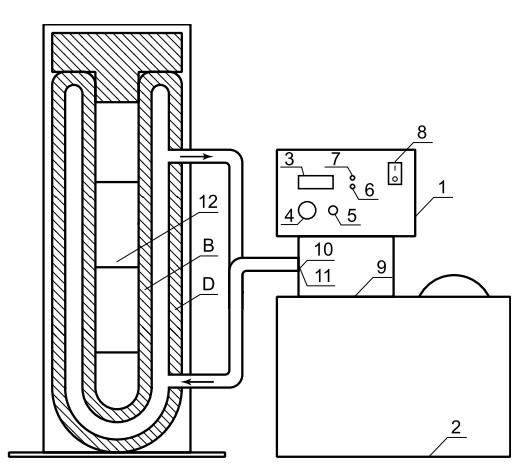
\includegraphics[width = 0.7\textwidth]{установка.jpg}
	\end{center}
	\caption{Установка для определения коэффициента вязкости жидкости}
\end{figure}

\section{Ход работы}

\begin{table}[h!]
\begin{tabular}{|l|clllll|}
\hline
T, К                                 & \multicolumn{1}{l|}{298}   & \multicolumn{1}{l|}{304}   & \multicolumn{1}{l|}{308}   & \multicolumn{1}{l|}{313}   & \multicolumn{1}{l|}{318}   & 323   \\ \hline
$\rho_0, \text{ г/см}^3$             & \multicolumn{1}{l|}{1,258} & \multicolumn{1}{l|}{1,256} & \multicolumn{1}{l|}{1,254} & \multicolumn{1}{l|}{1,252} & \multicolumn{1}{l|}{1,250} & 1,248 \\ \hline
L, см                                & \multicolumn{6}{c|}{$20,0 \pm 0,1$}                                                                                                                    \\ \hline
$\rho_\text{стекла}, \text{ г/см}^3$ & \multicolumn{6}{c|}{2,52}                                                                                                                              \\ \hline
$\rho_\text{стали}, \text{ г/см}^3$  & \multicolumn{6}{c|}{7,80}                                                                                                                              \\ \hline
\end{tabular}
\end{table}

\noindent 1. Отберем 12 стеклянных и 12 стальных шариков и с помощью микроскопа измерим их средние диаметры (см. Таблицу ниже). Погрешность измерения диаметра для стеклянных шариков примем $\sigma_{d1} = 0,1 \text{ мм}$, для стальных - $\sigma_{d2} = 0,3 \text{ мм}$.

\medskip

\noindent 2. Измерим установившиеся скорости падения шариков на $L = 20 \text{ см}, \sigma_L = 0,1 \text{ см}$ и вычислим вязкость. Погрешность измерения времени примем $\sigma_t = 0,2 \text{ с}$. Оценим также время релакации $\tau$ и путь релаксации $S = v_\text{уст} \tau$.

\begin{table}[h!]
\begin{tabular}{|l|llll|}
\hline
T,  K  & \multicolumn{4}{c|}{298}                                                                               \\ \hline
шарики & \multicolumn{1}{l|}{1 стекло} & \multicolumn{1}{l|}{2 стекло} & \multicolumn{1}{l|}{1 сталь} & 2 сталь \\ \hline
d, мм  & \multicolumn{1}{l|}{2,06}     & \multicolumn{1}{l|}{2,04}     & \multicolumn{1}{l|}{0,80}    & 0,80    \\ \hline
t, с   & \multicolumn{1}{l|}{47,03}    & \multicolumn{1}{l|}{47,22}    & \multicolumn{1}{l|}{50,50}   & 50,90   \\ \hline
\end{tabular}
\end{table}

\begin{table}[h!]
\begin{tabular}{|l|llll|}
\hline
T,  K  & \multicolumn{4}{c|}{304}                                                                               \\ \hline
шарики & \multicolumn{1}{l|}{1 стекло} & \multicolumn{1}{l|}{2 стекло} & \multicolumn{1}{l|}{1 сталь} & 2 сталь \\ \hline
d, мм  & \multicolumn{1}{l|}{2,02}     & \multicolumn{1}{l|}{2,10}     & \multicolumn{1}{l|}{0,82}    & 0,94    \\ \hline
t, с   & \multicolumn{1}{l|}{29,79}    & \multicolumn{1}{l|}{29,39}    & \multicolumn{1}{l|}{31,00}   & 32,52   \\ \hline
\end{tabular}
\end{table}



\begin{table}[h!]
\begin{tabular}{|l|llll|}
\hline
T,  K  & \multicolumn{4}{c|}{308}                                                                               \\ \hline
шарики & \multicolumn{1}{l|}{1 стекло} & \multicolumn{1}{l|}{2 стекло} & \multicolumn{1}{l|}{1 сталь} & 2 сталь \\ \hline
d, мм  & \multicolumn{1}{l|}{2,06}     & \multicolumn{1}{l|}{2,08}     & \multicolumn{1}{l|}{1,20}    & 0,80    \\ \hline
t, с   & \multicolumn{1}{l|}{23,81}    & \multicolumn{1}{l|}{23,06}    & \multicolumn{1}{l|}{26,36}   & 36,32   \\ \hline
\end{tabular}
\end{table}



\begin{table}[h!]
\begin{tabular}{|l|llll|}
\hline
T,  K  & \multicolumn{4}{c|}{313}                                                                               \\ \hline
шарики & \multicolumn{1}{l|}{1 стекло} & \multicolumn{1}{l|}{2 стекло} & \multicolumn{1}{l|}{1 сталь} & 2 сталь \\ \hline
d, мм  & \multicolumn{1}{l|}{2,12}     & \multicolumn{1}{l|}{2,10}     & \multicolumn{1}{l|}{0,72}    & 0,84    \\ \hline
t, с   & \multicolumn{1}{l|}{17,39}    & \multicolumn{1}{l|}{16,32}    & \multicolumn{1}{l|}{29,88}   & 17,88   \\ \hline
\end{tabular}
\end{table}



\begin{table}[h!]
\begin{tabular}{|l|llll|}
\hline
T,  K  & \multicolumn{4}{c|}{318}                                                                               \\ \hline
шарики & \multicolumn{1}{l|}{1 стекло} & \multicolumn{1}{l|}{2 стекло} & \multicolumn{1}{l|}{1 сталь} & 2 сталь \\ \hline
d, мм  & \multicolumn{1}{l|}{2,08}     & \multicolumn{1}{l|}{2,10}     & \multicolumn{1}{l|}{0,68}    & 0,82    \\ \hline
t, с   & \multicolumn{1}{l|}{12,08}    & \multicolumn{1}{l|}{12,04}    & \multicolumn{1}{l|}{24,74}   & 18,39   \\ \hline
\end{tabular}
\end{table}



\begin{table}[h!]
\begin{tabular}{|l|llll|}
\hline
T,  K  & \multicolumn{4}{c|}{323}                                                                               \\ \hline
шарики & \multicolumn{1}{l|}{1 стекло} & \multicolumn{1}{l|}{2 стекло} & \multicolumn{1}{l|}{1 сталь} & 2 сталь \\ \hline
d, мм  & \multicolumn{1}{l|}{2,06}     & \multicolumn{1}{l|}{2,06}     & \multicolumn{1}{l|}{0,76}    & 0,70    \\ \hline
t, с   & \multicolumn{1}{l|}{9,00}     & \multicolumn{1}{l|}{8,88}     & \multicolumn{1}{l|}{12,78}   & 15,52   \\ \hline
\end{tabular}
\end{table}

\noindent Получаем следующие значения:

\begin{table}[h!]
\begin{tabular}{|l|ll|ll|ll|ll|}
\hline
T, К                                    & \multicolumn{2}{c|}{298}            & \multicolumn{2}{c|}{304}            & \multicolumn{2}{c|}{308}            & \multicolumn{2}{c|}{313}            \\ \hline
$\eta, \text{Па} \cdot \text{с}$        & \multicolumn{2}{c|}{0,63}           & \multicolumn{2}{c|}{0,44}           & \multicolumn{2}{c|}{0,36}           & \multicolumn{2}{c|}{0,25}           \\ \hline
$\sigma_\eta, \text{Па} \cdot \text{с}$ & \multicolumn{2}{c|}{0,18}           & \multicolumn{2}{c|}{0,12}           & \multicolumn{2}{c|}{0,09}           & \multicolumn{2}{c|}{0,08}           \\ \hline
                                        & \multicolumn{1}{l|}{cтекло} & сталь & \multicolumn{1}{l|}{стекло} & сталь & \multicolumn{1}{l|}{стекло} & сталь & \multicolumn{1}{l|}{стекло} & сталь \\ \hline
$\tau, \cdot 10^{-3}\text{ с}$          & \multicolumn{1}{l|}{0,86}   & 0,48  & \multicolumn{1}{l|}{1,38}   & 0,77  & \multicolumn{1}{l|}{1,73}   & 1,21  & \multicolumn{1}{l|}{2,41}   & 1,09  \\ \hline
$\sigma_\tau, \cdot 10^{-3}\text{ с}$   & \multicolumn{1}{l|}{0,08}   & 0,12  & \multicolumn{1}{l|}{0,13}   & 0,11  & \multicolumn{1}{l|}{0,17}   & 0,14  & \multicolumn{1}{l|}{0,23}   & 0,16  \\ \hline
$S, \cdot 10^{-2}\text{ мм}$            & \multicolumn{1}{l|}{0,37}   & 0,19  & \multicolumn{1}{l|}{0,93}   & 0,48  & \multicolumn{1}{l|}{1,48}   & 0,84  & \multicolumn{1}{l|}{2,86}   & 1,03  \\ \hline
$\sigma_S, \cdot 10^{-2}\text{ мм}$     & \multicolumn{1}{l|}{0,04}   & 0,14  & \multicolumn{1}{l|}{0,09}   & 0,33  & \multicolumn{1}{l|}{0,14}   & 0,47  & \multicolumn{1}{l|}{0,04}   & 0,01  \\ \hline
\end{tabular}
\end{table}

\newpage

\begin{table}[h!]
\begin{tabular}{|l|ll|ll|}
\hline
T, К                                    & \multicolumn{2}{c|}{318}            & \multicolumn{2}{c|}{323}            \\ \hline
$\eta, \text{Па} \cdot \text{с}$        & \multicolumn{2}{c|}{0,20}           & \multicolumn{2}{c|}{0,13}           \\ \hline
$\sigma_\eta, \text{Па} \cdot \text{с}$ & \multicolumn{2}{c|}{0,07}           & \multicolumn{2}{c|}{0,04}           \\ \hline
                                        & \multicolumn{1}{l|}{стекло} & сталь & \multicolumn{1}{l|}{стекло} & сталь \\ \hline
$\tau, \cdot 10^{-3}\text{ с}$          & \multicolumn{1}{l|}{3,36}   & 1,15  & \multicolumn{1}{l|}{4,52}   & 1,73  \\ \hline
$\sigma_\tau, \cdot 10^{-3}\text{ с}$   & \multicolumn{1}{l|}{0,22}   & 0,13  & \multicolumn{1}{l|}{0,23}   & 0,24  \\ \hline
$S, \cdot 10^{-2}\text{ мм}$            & \multicolumn{1}{l|}{5,57}   & 1,12  & \multicolumn{1}{l|}{10,12}  & 2,50  \\ \hline
$\sigma_S, \cdot 10^{-2}\text{ мм}$     & \multicolumn{1}{l|}{0,10}   & 0,01  & \multicolumn{1}{l|}{1,04}   & 2,04  \\ \hline
\end{tabular}
\end{table}


\noindent 3. Для каждого из опытов вычислим значение числа $Re$.

\begin{table}[h!]
\begin{tabular}{|l|l|l|l|l|l|l|}
\hline
T, K & 298   & 304   & 308   & 313 & 318   & 323   \\ \hline
$Re$ & 0,006 & 0,014 & 0,022 & 0,040  & 0,070 & 0,134 \\ \hline
\end{tabular}
\end{table}

\noindent 4. Построим график зависимости ln$\eta$ от $1/T$ и по угловому коэффициенту прямой определим энергию активации.  

\begin{figure}[h!]
	\begin{center}
		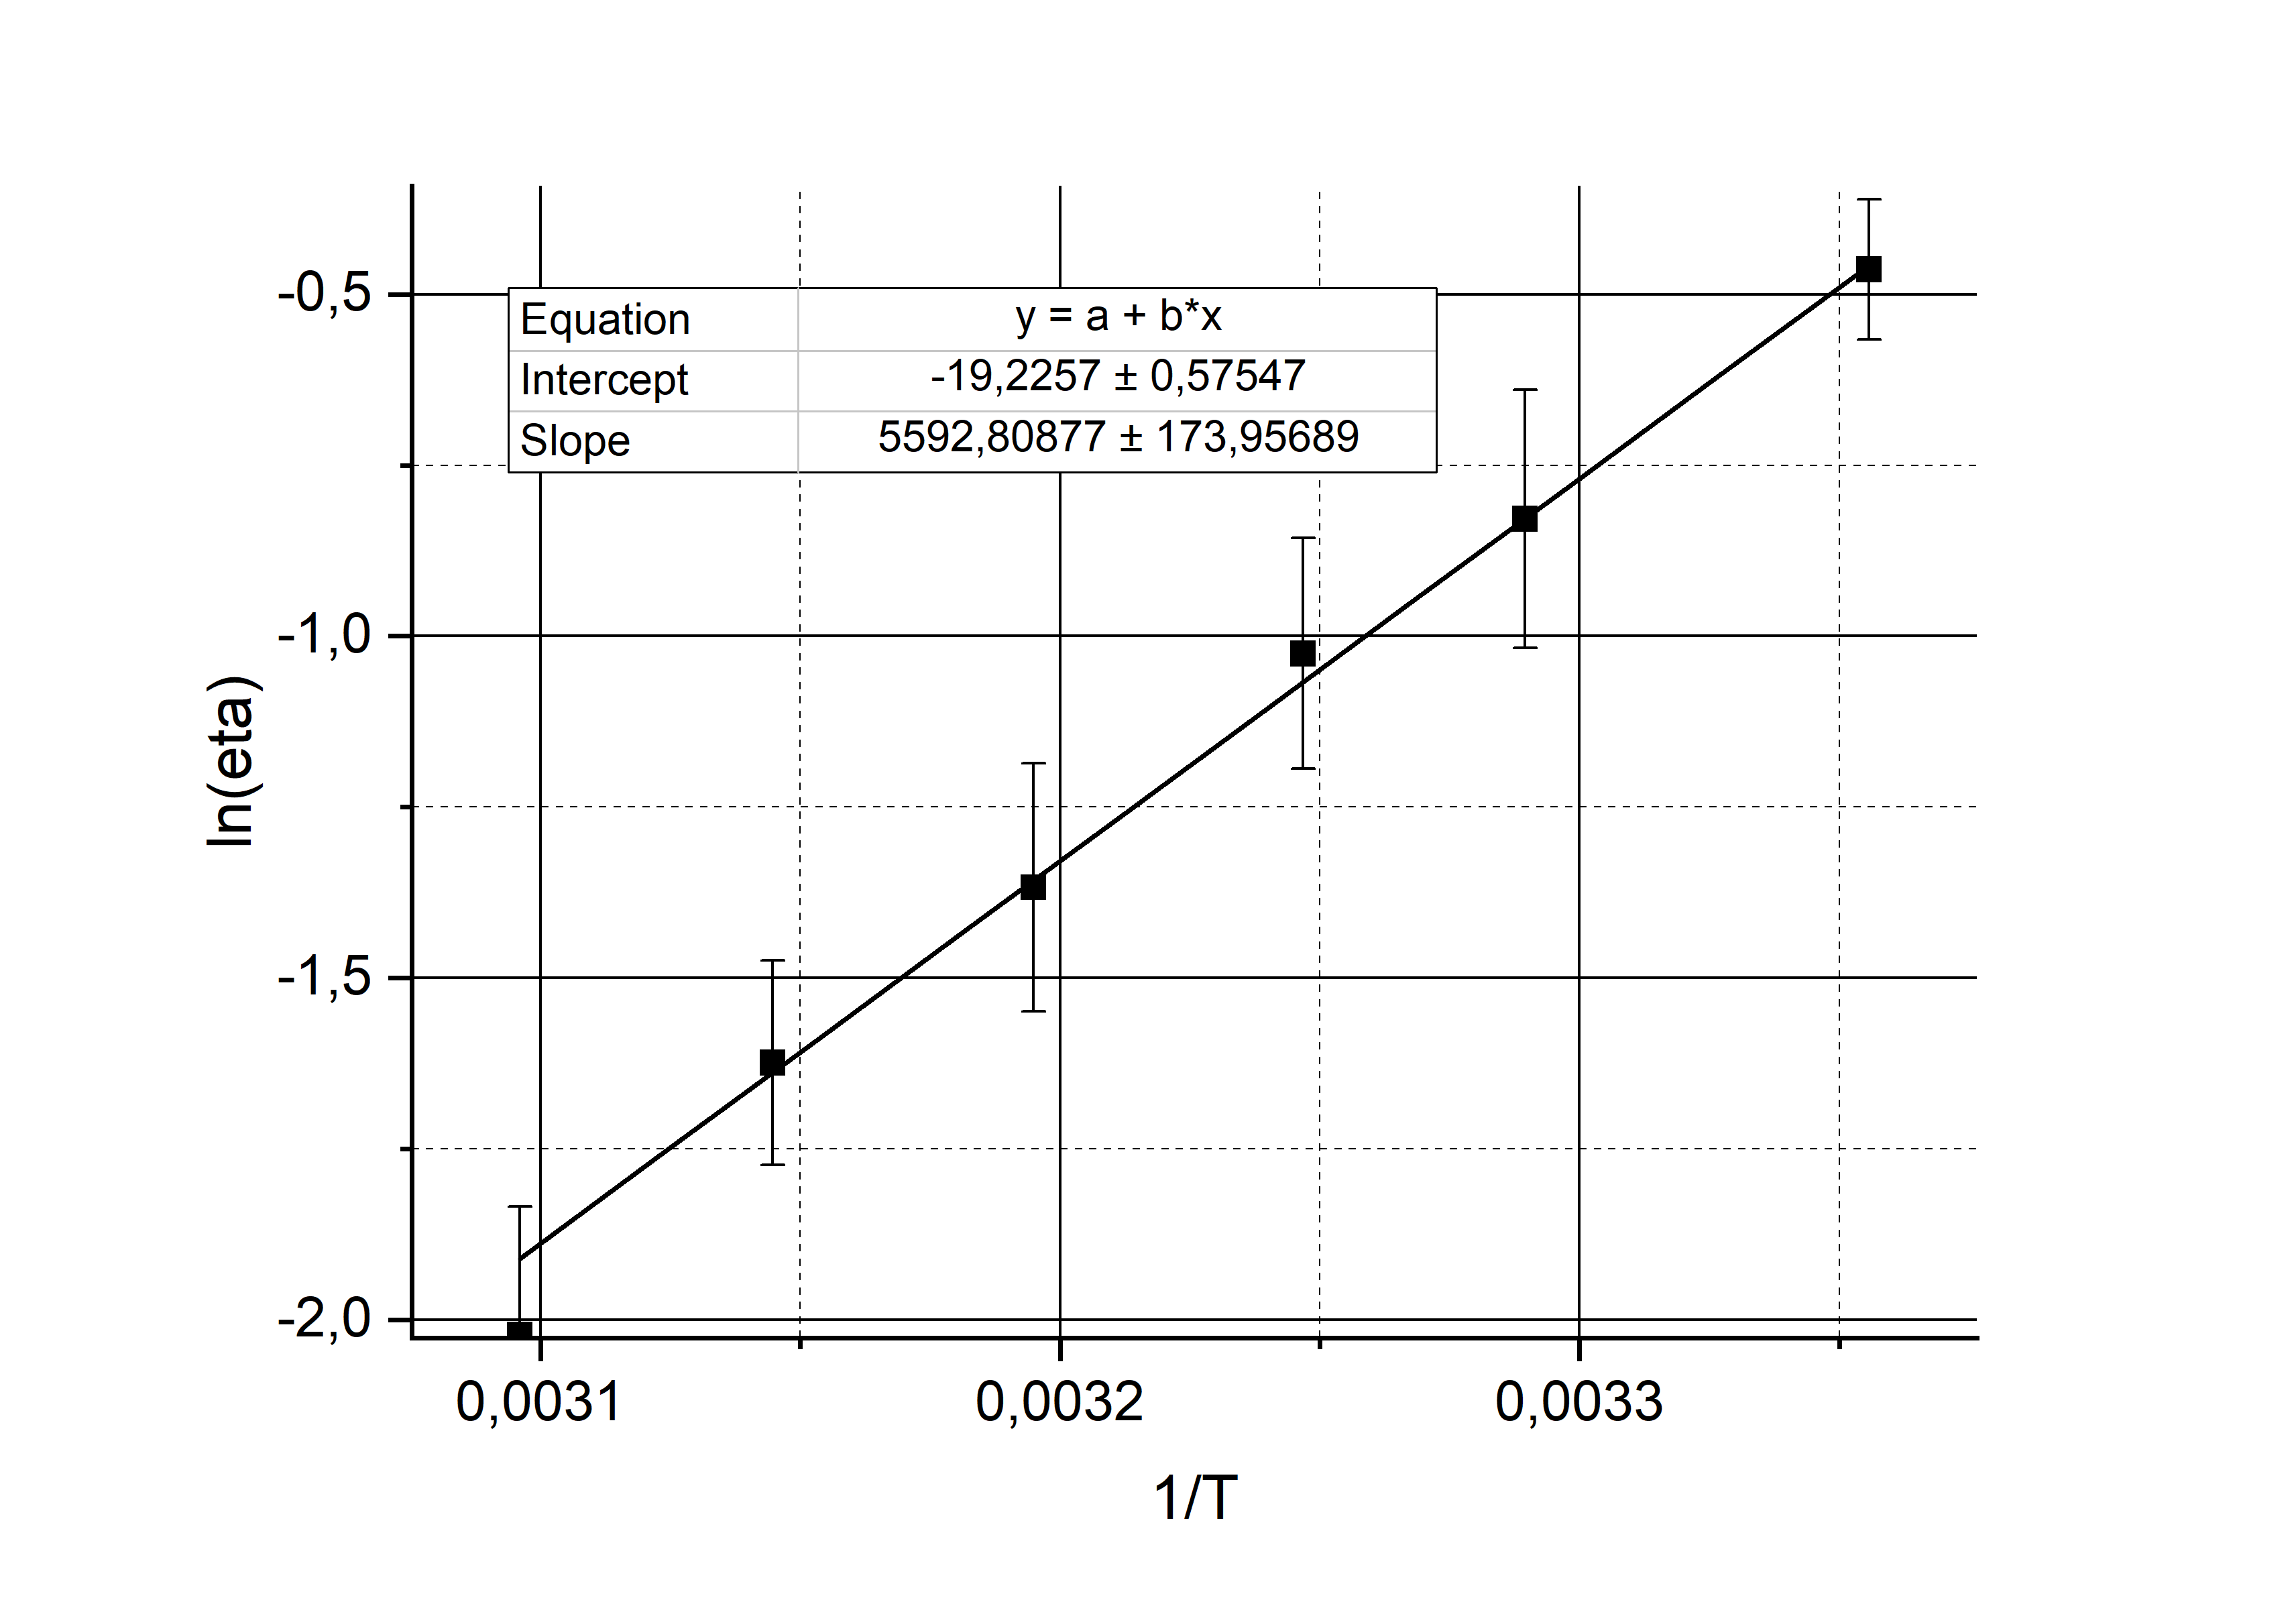
\includegraphics[width = 1\textwidth]{1.png}
	\end{center}
\end{figure}

\[
W = k \frac{d\ln\eta}{d(1/T)} = (7,7 \pm 0,2)\,\cdot 10^{-20}\ \text{Дж}
\]

\newpage

\section{Вывод}

\noindent В ходе работы:

\medskip

\noindent 1. Вычислена вязкость исследуемой жидкости по закону Стокса при различных температурах. Значения в пределах погрешности соответствуют табличным.

\begin{table}[h!]
\begin{tabular}{|l|l|l|l|l|l|l|}
\hline
T, К                                    & 298  & 304  & 308  & 313  & 318  & 323  \\ \hline
$\eta, \text{Па} \cdot \text{с}$        & 0,63 & 0,44 & 0,36 & 0,25 & 0,20 & 0,13 \\ \hline
$\sigma_\eta, \text{Па} \cdot \text{с}$ & 0,18 & 0,12 & 0,09 & 0,08 & 0,07 & 0,04 \\ \hline
\end{tabular}
\end{table}

\noindent 2. Получены значения времени релаксации. Поскольку время падения в несколько раз больше времени релаксации, процесс установления скорости можно считать закончившимся.

\medskip

\noindent 3. Вычислена энергия активации глицерина $W = (7,7 \pm 0,2)\,\cdot 10^{-20}\ \text{Дж}$.

\noindent 4. Получены числа Рейнольдса (все они меньше 0,5), которые позволяют утверждать, что в условиях опыта течение можно считать ламинарным.

\medskip 

\end{document}